
%  ========== PREAMBLE ==========

\documentclass[11pt]{article}

% -= Packages =-

\usepackage[top=1in,bottom=1in,left=1in,right=1in,paper=a4paper]{geometry}
\usepackage{graphicx,float}
\usepackage{hyperref}
\usepackage{tocloft}
\usepackage[immediate]{silence}
\WarningFilter[temp]{latex}{Command} % silence the warning
\usepackage{sectsty}
\DeactivateWarningFilters[temp] % So nothing unrelated gets silenced
\usepackage[most]{tcolorbox}
\usepackage{textcomp}
\usepackage{amsmath,amsfonts,amssymb,amsthm,mathtools,gensymb}
\usepackage{hyperref}
\usepackage{tikz}
\usepackage{titling}
\usepackage{lipsum}
\usepackage{mathtools}
\usepackage{enumitem}
\usepackage[utf8]{inputenc}
\usepackage[titletoc,title]{appendix}
\usepackage{xcolor}
\usepackage[twoside]{fancyhdr}
\usepackage[parfill]{parskip}
\usepackage{multicol}
\usepackage{pgfplots}
\pgfplotsset{compat=1.15}
\usepackage{mathrsfs}
\usetikzlibrary{arrows}
\usepackage{fontawesome5}
\usepackage{titlesec}

\usetikzlibrary{arrows.meta, decorations.pathreplacing,calc}

\makeatletter % disable the runtime redefinitions
\let\SS@makeulinesect\relax
\let\SS@makeulinepartchap\relax
\makeatother


% -= Settings =-

\pagestyle{fancy}
\allsectionsfont{\bfseries\sffamily}

\graphicspath{ {./images/} }

\hypersetup{
    colorlinks,
    citecolor=black,
    filecolor=black,
    linkcolor=purple,
    urlcolor=blue
}


\renewcommand{\baselinestretch}{1.5}
\newcommand{\qedblack}{$\hfill\blacksquare$}

\newcommand{\divides}{\mid}
\newcommand{\notdivides}{\nmid}

\DeclareMathOperator{\ord}{ord}

\DeclarePairedDelimiter\abs{\lvert}{\rvert}%
\DeclarePairedDelimiter\norm{\lVert}{\rVert}%
\DeclareMathOperator{\lcm}{lcm}

\renewcommand{\footrulewidth}{0.45pt}
\renewcommand{\headrulewidth}{0.45pt}
\definecolor{bbe}{HTML}{000000}
\definecolor{headerbg}{RGB}{0, 0, 0} 
\definecolor{headertext}{RGB}{255, 250, 240}
\definecolor{mahdarkblue}{HTML}{1e3f66}
\definecolor{mahdarknavy}{HTML}{254a6d}
\definecolor{mahnavy}{HTML}{2e5984}
\definecolor{mahblue}{HTML}{528aae}
\definecolor{mahlightblue}{HTML}{73a5c6}
\definecolor{mahsky}{HTML}{91bad6}
\definecolor{mahturquoise}{HTML}{5f8998}
\setlength{\headheight}{21pt}


% -= Theorem Environments =-

\newtcolorbox[auto counter,number within=section,number format=\arabic]{definition}[1][]{
            colback=mahdarkblue!10!white,enhanced,
            title={\textbf{\faBook\ \ Định nghĩa~\thetcbcounter}},
            attach boxed title to top left={xshift=-4mm},
            boxrule=0pt,
            after skip=1cm,before skip=1cm,right skip=0cm,
            breakable,fonttitle=\sffamily,
            toprule=0pt,bottomrule=0pt,rightrule=0pt,leftrule=4pt,
            arc=0mm,
            skin=enhancedlast jigsaw,
            sharp corners,
            colframe=mahdarkblue,colbacktitle=mahdarkblue!90!white,
            boxed title style={
                frame code={
                    \fill[mahdarkblue!90!white](frame.south west)--(frame.north west)--(frame.north east)--([xshift=3mm]frame.east)--(frame.south east)--cycle;
                    \draw[line width=1mm,mahdarkblue!90!white]([xshift=2mm]frame.north east)--([xshift=5mm]frame.east)--([xshift=2mm]frame.south east);
                    \draw[line width=1mm,mahdarkblue!90!white]([xshift=5mm]frame.north east)--([xshift=8mm]frame.east)--([xshift=5mm]frame.south east);
                    \fill[mahdarkblue!80!white](frame.south west)--+(4mm,-2mm)--+(4mm,2mm)--cycle;
                }
            }
}

\newtcolorbox[auto counter,number within=section,number format=\arabic]{theorem}[1][]{
            colback=mahdarknavy!10!white,enhanced,
            title={\textbf{\faPen\ \ Định lí~\thetcbcounter}},
            attach boxed title to top left={xshift=-4mm},
            boxrule=0pt,
            after skip=1cm,before skip=1cm,right skip=0cm,
            breakable,fonttitle=\sffamily,
            toprule=0pt,bottomrule=0pt,rightrule=0pt,leftrule=4pt,
            arc=0mm,
            skin=enhancedlast jigsaw,
            sharp corners,
            colframe=mahdarknavy,colbacktitle=mahdarknavy!90!white,
            boxed title style={
                frame code={
                    \fill[mahdarknavy!90!white](frame.south west)--(frame.north west)--(frame.north east)--([xshift=3mm]frame.east)--(frame.south east)--cycle;
                    \draw[line width=1mm,mahdarknavy!90!white]([xshift=2mm]frame.north east)--([xshift=5mm]frame.east)--([xshift=2mm]frame.south east);
                    \draw[line width=1mm,mahdarknavy!90!white]([xshift=5mm]frame.north east)--([xshift=8mm]frame.east)--([xshift=5mm]frame.south east);
                    \fill[mahdarknavy!80!white](frame.south west)--+(4mm,-2mm)--+(4mm,2mm)--cycle;
                }
            }
}

\newtcolorbox[auto counter,number within=section,number format=\arabic]{property}[1][]{
            colback=mahnavy!10!white,enhanced,
            title={\textbf{\faBookmark\ \ Tính chất~\thetcbcounter}},
            attach boxed title to top left={xshift=-4mm},
            boxrule=0pt,
            after skip=1cm,before skip=1cm,right skip=0cm,
            breakable,fonttitle=\sffamily,
            toprule=0pt,bottomrule=0pt,rightrule=0pt,leftrule=4pt,
            arc=0mm,
            skin=enhancedlast jigsaw,
            sharp corners,
            colframe=mahnavy,colbacktitle=mahnavy!90!white,
            boxed title style={
                frame code={
                    \fill[mahnavy!90!white](frame.south west)--(frame.north west)--(frame.north east)--([xshift=3mm]frame.east)--(frame.south east)--cycle;
                    \draw[line width=1mm,mahnavy!90!white]([xshift=2mm]frame.north east)--([xshift=5mm]frame.east)--([xshift=2mm]frame.south east);
                    \draw[line width=1mm,mahnavy!90!white]([xshift=5mm]frame.north east)--([xshift=8mm]frame.east)--([xshift=5mm]frame.south east);
                    \fill[mahnavy!80!white](frame.south west)--+(4mm,-2mm)--+(4mm,2mm)--cycle;
                }
            }
}

\newtcolorbox[auto counter,number format=\arabic]{problem}[1][]{
            colback=mahblue!10!white,enhanced,
            title={\textbf{\faFile*\ \ Problem~\thetcbcounter}},
            attach boxed title to top left={xshift=-4mm},
            boxrule=0pt,
            after skip=1cm,before skip=1cm,right skip=0cm,
            breakable,fonttitle=\sffamily,
            toprule=0pt,bottomrule=0pt,rightrule=0pt,leftrule=4pt,
            arc=0mm,
            skin=enhancedlast jigsaw,
            sharp corners,
            colframe=mahblue,colbacktitle=mahblue!90!white,
            boxed title style={
                frame code={
                    \fill[mahblue!90!white](frame.south west)--(frame.north west)--(frame.north east)--([xshift=3mm]frame.east)--(frame.south east)--cycle;
                    \draw[line width=1mm,mahblue!90!white]([xshift=2mm]frame.north east)--([xshift=5mm]frame.east)--([xshift=2mm]frame.south east);
                    \draw[line width=1mm,mahblue!90!white]([xshift=5mm]frame.north east)--([xshift=8mm]frame.east)--([xshift=5mm]frame.south east);
                    \fill[mahblue!80!white](frame.south west)--+(4mm,-2mm)--+(4mm,2mm)--cycle;
                }
            }
}

\newtcolorbox[auto counter,number within=section,number format=\arabic]{problemme}[1][]{
            colback=mahblue!10!white,enhanced,
            title={\textbf{\faFile*\ \ Problem statement}},
            attach boxed title to top left={xshift=-4mm},
            boxrule=0pt,
            after skip=1cm,before skip=1cm,right skip=0cm,
            breakable,fonttitle=\sffamily,
            toprule=0pt,bottomrule=0pt,rightrule=0pt,leftrule=4pt,
            arc=0mm,
            skin=enhancedlast jigsaw,
            sharp corners,
            colframe=mahblue,colbacktitle=mahblue!90!white,
            boxed title style={
                frame code={
                    \fill[mahblue!90!white](frame.south west)--(frame.north west)--(frame.north east)--([xshift=3mm]frame.east)--(frame.south east)--cycle;
                    \draw[line width=1mm,mahblue!90!white]([xshift=2mm]frame.north east)--([xshift=5mm]frame.east)--([xshift=2mm]frame.south east);
                    \draw[line width=1mm,mahblue!90!white]([xshift=5mm]frame.north east)--([xshift=8mm]frame.east)--([xshift=5mm]frame.south east);
                    \fill[mahblue!80!white](frame.south west)--+(4mm,-2mm)--+(4mm,2mm)--cycle;
                }
            }
}

\newtcolorbox[auto counter,number format=\arabic]{exproblem}[1][]{
            colback=mahblue!10!white,enhanced,
            title={\textbf{\faFile*\ \ Ví dụ~\thetcbcounter}},
            attach boxed title to top left={xshift=-4mm},
            boxrule=0pt,
            after skip=1cm,before skip=1cm,right skip=0cm,
            breakable,fonttitle=\sffamily,
            toprule=0pt,bottomrule=0pt,rightrule=0pt,leftrule=4pt,
            arc=0mm,
            skin=enhancedlast jigsaw,
            sharp corners,
            colframe=mahblue,colbacktitle=mahblue!90!white,
            boxed title style={
                frame code={
                    \fill[mahblue!90!white](frame.south west)--(frame.north west)--(frame.north east)--([xshift=3mm]frame.east)--(frame.south east)--cycle;
                    \draw[line width=1mm,mahblue!90!white]([xshift=2mm]frame.north east)--([xshift=5mm]frame.east)--([xshift=2mm]frame.south east);
                    \draw[line width=1mm,mahblue!90!white]([xshift=5mm]frame.north east)--([xshift=8mm]frame.east)--([xshift=5mm]frame.south east);
                    \fill[mahblue!80!white](frame.south west)--+(4mm,-2mm)--+(4mm,2mm)--cycle;
                }
            }
}

\newtcolorbox[auto counter,number within=section,number format=\arabic]{corollary}[1][]{
            colback=mahlightblue!10!white,enhanced,
            title={\textbf{\faHandPointRight[regular] \ \ Hệ quả \thetcbcounter}},
            boxrule=0pt,
	    frame hidden,
            breakable,fonttitle=\sffamily,
            arc=0mm,
            sharp corners,
            detach title,
            before upper = \tcbtitle\par\smallskip,
            colframe=mahlightblue,coltitle=mahlightblue!85!black,
            borderline west = {1mm}{0pt}{mahlightblue!85!black},
            segmentation style={solid, mahlightblue!85!black}
}

\newtcolorbox[auto counter,number format=\arabic]{lemma}[1][]{
            colback=mahlightblue!10!white,enhanced,
            title={\textbf{\faBook \ \ Bổ đề}},
            boxrule=0pt,
	    frame hidden,
            breakable,fonttitle=\sffamily,
            arc=0mm,
            sharp corners,
            detach title,
            before upper = \tcbtitle\par\smallskip,
            colframe=mahlightblue,coltitle=mahlightblue!85!black,
            borderline west = {1mm}{0pt}{mahlightblue!85!black},
            segmentation style={solid, mahlightblue!85!black}
}

\newtcolorbox[auto counter,number format=\arabic]{claim}[1][]{
            colback=mahturquoise!10!white,enhanced,
            title={\textbf{\faExclamation \ \ Claim --- \ }},
            boxrule=0pt,
	    frame hidden,
            breakable,fonttitle=\sffamily,
            arc=0mm,
            sharp corners,
            detach title,
            before upper = \tcbtitle,
            colframe=mahturquoise,coltitle=mahturquoise!85!black,
            borderline west = {1mm}{0pt}{mahturquoise!85!black},
            segmentation style={solid, mahturquoise!85!black}
}

\newtcolorbox[auto counter,number format=\arabic]{remark}[1][]{
            colback=mahsky!10!white,enhanced,
            title={\textbf{\faExclamation \ \ Remark --- \ }},
            boxrule=0pt,
	    frame hidden,
            breakable,fonttitle=\sffamily,
            arc=0mm,
            sharp corners,
            detach title,
            before upper = \tcbtitle,
            colframe=mahsky,coltitle=mahsky!85!black,
            borderline west = {1mm}{0pt}{mahsky!85!black},
            segmentation style={solid, mahsky!85!black}
}

\newtcolorbox[auto counter,number format=\arabic]{motivation}[1][]{
            colback=mahlightblue!10!white,enhanced,
            title={\textbf{\faQuestion \ \ Motivation}},
            boxrule=0pt,
	    frame hidden,
            breakable,fonttitle=\sffamily,
            arc=0mm,
            sharp corners,
            detach title,
            before upper = \tcbtitle\par\smallskip,
            colframe=mahlightblue,coltitle=mahlightblue!85!black,
            borderline west = {1mm}{0pt}{mahlightblue!85!black},
            segmentation style={solid, mahlightblue!85!black}
}

\newenvironment{solution}[1][Solution]{%
  \proof[\normalfont \faPenNib \hspace{0.2cm} \ttfamily \scshape \large #1]%
}{\(\hfill \blacksquare\){\parfillskip0pt\par}}

\theoremstyle{definition}
\newtheorem{exercise}{Problem}

\newcommand{\boom}{\vspace{0.25cm}}


% -= Header + Title =-

% Header

\fancyhead[RO]{\footnotesize \thepage}
\fancyhead[RE]{\footnotesize \textsc{VMO 2014 Solution Notes}}
\fancyhead[LE]{\footnotesize \thepage}
\fancyhead[LO]{\footnotesize \scshape Mark Nguyen}
\fancyfoot{}

\renewcommand{\footrulewidth}{0pt}

% Section title

\makeatletter
\titleformat{\section}
  {\normalfont\Large\bfseries\sffamily}{\color{purple}\S\thesection}{1em}{}
\titleformat{\subsection}
  {\normalfont\large\bfseries\sffamily}{\color{purple}\S\thesubsection}{1em}{}
\titleformat{\subsubsection}
  {\normalfont\normalsize\bfseries\ttfamily}{\color{purple}\S\thesubsubsection}{1em}{}
\makeatother
  

\renewcommand{\cfttoctitlefont}{\hfill\bfseries\LARGE}
\renewcommand{\cftaftertoctitle}{\hfill\hspace{-1cm}}

\title{\textbf{\Huge VMO 2014 Solution Notes}}
\author{\LARGE \textsc{Mark Nguyen}}
\date{\sffamily\today}

\begin{document}

\maketitle

\begin{abstract}
    This document compiles my solutions and best attempts for the 2014 Vietnamese Mathematical Olympiad. While I originally considered writing in Vietnamese, I chose English to make it accessible to a wider audience and to refine my language skills. All content is authored and maintained by me. Comments and corrections are welcome.
\end{abstract}

\tableofcontents

\newpage

\section{Problems}

    \subsection*{Day 1}

        \begin{exercise}
            Given two sequences \((x_n)_{n=1}^{+\infty}\) and \((y_n)_{n=1}^{+\infty}\) of positive real numbers, defined by \(x_1 = 1\), \(y_1 = \sqrt{3}\), and for all positive integers \(n\),
            \[\begin{cases}
                x_{n+1}y_{n+1} - x_n = 0 \\
                x_{n+1}^2 + y_n = 2
            \end{cases}.\]
            Prove that \((x_n)_{n=1}^{+\infty}\) and \((y_n)_{n=1}^{+\infty}\) converges, then find \(\lim\limits_{n \to +\infty} x_n\) and \(\lim\limits_{n \to +\infty} y_n\).
        \end{exercise}
    
        \boom
    
        \begin{exercise}
            Prove that for all positive integers \(n\), the polynomial
            \[P(x) = (x^2 - 7x + 6)^{2n} + 13\]
            cannot be written as the product of \(n + 1\) non-constant polynomials with integer coefficients.
        \end{exercise}
    
        \boom
    
        \begin{exercise}
            Given a regular 103-sided polygon with 79 vertices colored red and the remaining vertices colored blue. Denote \(A\) as the number of pairs of adjacent red vertices, and \(B\) as the number of pairs of adjacent blue vertices.
            \begin{enumerate}
                \item[(a)] Find all possible values of \((A,B)\).
                \item[(b)] Two ways of colorings of the polygon are called \emph{similar} if one of them can be obtained from another through rotation at the circumcenter of the regular polygon. Determine the number of pairwise non-similar colorings of the polygon satisfying \(B = 14\).
            \end{enumerate}
        \end{exercise}
    
        \boom
    
        \begin{exercise}
            Let \(ABC\) be an acute and scalene triangle (\(AB < AC)\)) with circumcircle \((O)\). Let \(I\) be the midpoint of arc \(BC\) not containing \(A\) of circle \((O)\). Let \(K\) be a point on \(AC\) (\(K \neq C\)) such that \(IK = IC\). Line \(BK\) intersects \((O)\) at \(D\) (\(D \neq B\)) and intersects \(AI\) at \(E\). \(DI\) intersects \(AC\) at \(F\).
            \begin{enumerate}
                \item[(a)] Prove that \(EF = \dfrac{BC}{2}\).
                \item[(b)] Let \(M\) be a point on \(DI\) satisfies \(CM\) is parallel to \(AD\). Line \(KM\) intersects \(BC\) at \(N\), and the circumcircle of triangle \(BKN\) intersects \((O)\) at \(P\) (\(P \neq B\)). Prove that \(PK\) passes through the midpoint of segment \(AD\).
            \end{enumerate}
        \end{exercise}

    \newpage
    
    \subsection*{Day 2}

        \begin{exercise}
            Given a fixed circle \((O)\), \(B\) and \(C\) are fixed points on \((O)\), and \(A\) is a moving point on \((O)\) such that \(ABC\) is an acute, scalene triangle. Point \(M\), \(N\) lies on ray \(AB\), \(AC\) respectively, such that \(MA = MC\) and \(NA = NB\). Let \(P\) be the intersection of circles \((AMN)\) and \((O)\), and \(Q\) be the intersection of lines \(MN\) and \(BC\).
            \begin{enumerate}
                \item[(a)] Prove that \(A\), \(P\), and \(Q\) are collinear.
                \item[(b)] Let \(D\) be the midpoint of segment \(BC\), \(K\) be the intersection of circles \((M;MA)\) and \((N;NA)\) (\(K \neq A\)). The line passing through \(A\) perpendicular to \(AK\) intersects \(BC\) at \(E\). The circumcircle of triangle \(ADE\) intersects \((O)\) at \(F\) (\(F \neq A\)). Prove that \(AF\) passes through a fixed point as \(A\) moves on \((O)\).
            \end{enumerate}
        \end{exercise}
    
        \boom
    
        \begin{exercise}
            Let \(x\), \(y\), and \(z\) be positive real numbers. Find the maximum value of the expression
            \[\frac{x^3y^4z^3}{(x^4 + y^4)(xy + z^2)^3} + \frac{y^3z^4x^3}{(y^4 + z^4)(yz + x^2)^3} + \frac{z^3x^4y^3}{(z^4 + x^4)(zx + y^2)^3}.\]
        \end{exercise}
    
        \boom
    
        \begin{exercise}
            Find all ordered sets of 2014 rational numbers, not necessarily distinct, such that if an arbitrary number in the set is removed, one can always partite the remaining 2013 numbers into 3 sets, such that each set has exactly 671 elements, and the product of all elements in each sets are all equal.
        \end{exercise}

    \newpage

\section{Solutions}

    \subsection{Solutions for Day 1}

        \begin{problem}
            Given two sequences \((x_n)_{n=1}^{+\infty}\) and \((y_n)_{n=1}^{+\infty}\) of positive real numbers, defined by \(x_1 = 1\), \(y_1 = \sqrt{3}\), and for all positive integers \(n\),
            \[\begin{cases}
                x_{n+1}y_{n+1} - x_n = 0 \\
                x_{n+1}^2 + y_n = 2
            \end{cases}.\]
            Prove that \((x_n)_{n=1}^{+\infty}\) and \((y_n)_{n=1}^{+\infty}\) converges, then find \(\lim\limits_{n \to +\infty} x_n\) and \(\lim\limits_{n \to +\infty} y_n\).
        \end{problem}

        \begin{solution}
            We make the following claim.
            
            \begin{claim}
                \(x_n^2 + y_n^2 = 4\), \(\forall n \in \mathbb{Z}^+\).
            \end{claim}
            
            \begin{motivation}
                We calculate the first 3 terms of each sequence
                \[x_2 = \sqrt{2 - \sqrt{3}} \text{, } y_2 = \sqrt{2 + \sqrt{3}} \text{;}\]
                \[x_3 = \sqrt{2 - \sqrt{2 + \sqrt{3}}} \text{, } y_3 = \sqrt{2 + \sqrt{2 + \sqrt{3}}}.\]
                It's easy to see \(x_2^2 + y_2^2 = x_3^2 + y_3^2 = 4\), and we thus can hypothesize the above claim.
            \end{motivation}

            \begin{proof}
                The base case where \(n = 1\) is trivial. Assume, for sake of induction, that the above claim holds true for every positive integer \(k \leq n\). Then we have
                \[x_{n+1}^2 + y_{n+1}^2 = 2 - y_n + \frac{x_n^2}{x_{n+1}^2} = 2 - y_n + \frac{4 - y_n^2}{2 - y_n} = 4.\]
                Thus the statement is also true for the \((n + 1)\)-th terms. By the induction principle, the claim is true for all \(n \in \mathbb{Z}^+\).
            \end{proof}

            From the above claim, we get \(y_n = \sqrt{4 - x_n^2} = \sqrt{2 + y_{n-1}}\) and \(x_n = \sqrt{4 - y_n^2} = \sqrt{2 - {y_{n-1}}}\).

            \begin{claim}
                \((y_n)\) converges to 2.
            \end{claim}

            \begin{proof}
                From the equation \(x_{n+1}^2 + y_n = 2\), since \(x_{n+1}^2 \geq 0\) we get \(y_n \leq 2\), or \((y_n)\) has an upper bound. Also, observe that
                \[y_n - y_{n-1} = \sqrt{2 + y_{n-1}} - y_{n-1} = \frac{2}{\sqrt{2 - y_{n=1}} + y_{n-1}} > 0 \text{, } \forall n \in \mathbb{Z}^+.\]
                Therefore, \((y_n)\) is strictly increasing. By Weierstrass' extreme value theorem, the sequence \((y_n)\) must have a limit. Denote \(L = \lim\limits_{n \to +\infty} y_n\). Since \((y_n)\) is a sequence of positive reals, \(L\) must be positive. As \(n \to +\infty\), the recursion equation for \((y_n)\) becomes
                \[L = \sqrt{2 + L} \implies L^2 - L - 2 = 0 \implies L = 2.\]
                Ergo, \((y_n)\) converges to 2 as \(n \to +\infty\).
            \end{proof}

            \begin{claim}
                \((x_n)\) converges to 0.
            \end{claim}

            \begin{proof}
                Since \((x_n)\) is a sequence of positive reals, \(x_n > 0\) for all \(n\), or \((x_n)\) has a lower bound. Also, observe that
                \[x_n - x_{n-1} = \sqrt{2 - y_{n-1}} - \sqrt{2 - y_{n-2}} = \frac{y_{n-2} - y_{n-1}}{\sqrt{2 - y_{n-1}} + \sqrt{2 - y_{n-2}}} < 0 \text{, } \forall n \in \mathbb{Z}^+.\]
                Therefore, \((x_n)\) is strictly decreasing. By Weierstrass' extreme value theorem, the sequence \((x_n)\) must have a limit. By the previous claim, \(\lim\limits_{n \to +\infty} y_n = 2\), so
                \[\lim\limits_{n \to +\infty} x_n = \lim\limits_{n \to +\infty} \sqrt{2 - y_{n-1}} = 0.\]
                Hence, \((x_n)\) converges to 0 as \(n \to +\infty\).
            \end{proof}

            Therefore, \(\lim\limits_{n \to +\infty} x_n = 0\) and \(\lim\limits_{n \to +\infty} y_n = 2\).
        \end{solution}

        \newpage

        \begin{problem}
            Prove that for all positive integers \(n\), the polynomial
            \[P(x) = (x^2 - 7x + 6)^{2n} + 13\]
            cannot be written as the product of \(n + 1\) non-constant polynomials with integer coefficients.
        \end{problem}

        \begin{solution}
            Assume, for sake of contradiction, that \(P(x)\) can be written as the product of \(n + 1\) non-constant polynomials \(P_1(x)\), \(P_2(x)\), \dots, \(P_{n+1}(x)\) with integer coefficients. Notice that \(P(x)\) is a monic polynomial (with the coefficient of the highest degree term equals 1) and \(\deg P = \deg \prod\limits_{i=1}^{n+1}P_i(x) = 4n\). We first take note of the degree of each individual polynomials.\\
            We need the following theorem.

            \begin{claim}
                Every polynomial with an odd degree must have a real root.
            \end{claim}

            \begin{proof}
                This theorem is well known, but we will give a sketch of a proof here for less ambiguity. Take the polynomial \(Q(x) = x^{2n+1} + a_{2n}x^{2n} + a_{2n-1}x^{2n-1} + \dots + a_0\). Divide both sides by \(x^{2n+1}\) and observe that for any \(\varepsilon > 0\), there exists \(N > 0\) such that for all \(\left|x\right| > N\), we have \(\left|\sum\limits_{k=0}^{2n} a_kx^{k-(2n+1)}\right| < \varepsilon\), so \(Q(x) > 0\). Similarly \(Q(x) < 0\) for all \(x < -N\). Intermediate value theorem implies there exists a real root.
            \end{proof}

            Now, assume, for sake of contradiction, that there exists a \(k \in \{1,2,\dots,n+1\}\) such that the polynomial \(P_k(x)\) has an odd degree. By the above theorem, \(P_k(x)\) must have a real root. But \(P(x) \geq 13 > 0\), \(\forall x \in \mathbb{R}\), so this is a contradiction. Therefore, \(2 \divides \deg P_i\), \(\forall i = \overline{1,n+1}\).\\
            By the pigeonhole principle, there exists at least 2 polynomials, each has the degree of 2. WLOG, let them be \(P_1(x)\) and \(P_2(x)\). Since \(P(x)\) is monic, let \(P_1(x) = x^2 + a_1x + b_1\) and \(P_2(x) = x^2 + a_2x + b_2\). Now, we have
            \[13 = P(1) = P_1(1) \cdot P_2(1) \cdots P_{n+1}(1) \text{ \ and \ } 13 = P(6) = P_1(6) \cdot P_2(6) \cdots P_{n+1}(6).\]
            Since \(P_i(x)\) are non-constant polynomials with integer coefficients, we must have \(P_i(x) \in \mathbb{Z}\) with \(x\) being an integer. From the first equation, we see that either \(P_1(x)\) or \(P_2(x)\) equals 1. WLOG let it be \(P_1(x) = 1\), implies \(a_1 = -b_1 = c\). So \(P_1(6) = 36 + 5c = 13\) or \(1\), thus obtain \(c = -7\), since \(c \in \mathbb{Z}\). Therefore \(P_1(x) = x^2 - 7x + 7\). This polynomial has 2 real roots, contradiction.\\
            Hence, \(P(x)\) cannot be written as what we wanted.
        \end{solution}

        \newpage

        \begin{problem}
            Given a regular 103-sided polygon with 79 vertices colored red and the remaining vertices colored blue. Denote \(A\) as the number of pairs of adjacent red vertices, and \(B\) as the number of pairs of adjacent blue vertices.
            \begin{enumerate}
                \item[(a)] Find all possible values of \((A,B)\).
                \item[(b)] Two ways of colorings of the polygon are called \emph{similar} if one of them can be obtained from another through rotation at the circumcenter of the regular polygon. Determine the number of pairwise non-similar colorings of the polygon satisfying \(B = 14\).
            \end{enumerate}
        \end{problem}
        
        \begin{solution}
            We define a red "bundle" is a set of adjacent vertices colored red, containing at least 1 red vertex, and similarly for blue bundles.
            \begin{enumerate}
                \item[(a)] There are \(103 - 79 = 24\) blue vertices. Notice that when all 79 red vertices are adjacent to each other, the number of pairs of adjacent red vertices equals 78. If these 79 vertices are split into 2 bundles, the number of pairs are 77, and so on. In other words, if there are \(c\) red bundles on the polygon, then the number of red pairs are \(79 - c\).\\
                If there are \(c\) red bundles, then there are also \(c\) blue bundles. Similar logic shows that there are \(24 - c\) blue pairs if there are \(c\) blue bundles. Since \(c\) can be any value from 1 to 24, there are a total of 24 possible values \((A,B)\) in the form of \((79 - c, 24 - c)\).

                \item[(b)] Since \(B = 14\), by the above logic this is equivalent to having 10 blue bundles on the polygon. We will count how many ways we can split 24 blue vertices into 10 bundles.\\
                Denote \(x_1\), \(x_2\), \dots, \(x_{10}\) as the number of blue vertices in each bundle 1, 2, \dots, 10, and \(y_n = \sum\limits_{i=1}^n x_i\), for all \(n = \overline{1,9}\) (we do not need to consider \(y_{10}\), since \(y_{10} = 24\) is a constant). With the condition \(1 \leq y_1 < y_2 < \dots < y_9 \leq 23\), we count how many possible values of \((y_1, y_2, \dots, y_9)\) are there. Indeed, there are \(\dbinom{23}{9}\) possible values.

                \begin{motivation}
                    The above statement is a formalization of the following observation: to count how many ways we can split up 24 blue vertices into 10 barriers is equivalent to count how many ways we can insert 9 entities (we will call it "barriers" for now) into the gaps between these 24 vertices. There are 23 gaps, so \(\dbinom{23}{9}\) there is.
                \end{motivation}

                Since there are 10 blue bundles, the number of red bundles must equal to 10. We will also count how many ways we can split 79 red vertices into 10 bundles. By similar logic, we can show that there are \(\dbinom{78}{9}\) possible ways.\\
                Now, we will begin distributing these 10 red bundles and 10 blue bundles on our polygon.
                \begin{center}
                    \textcolor{blue}{B B \dots \ B B} \textcolor{red}{R R \dots \ R R} \textcolor{blue}{B B \dots \ B B} \textcolor{red}{R R \dots \ R R} \textcolor{blue}{B B \dots \ B B} \dots \ \textcolor{red}{R R} \\
                \end{center}
                Without loss of generality, each way of coloring starts with the first vertex of the first blue bundle (since the case of the first vertex being any other vertex is similar to our case in consideration). Since 79 is a prime, each way of spliting red vertices into bundles is unique. On our polygon, we first add a blue bundle as our initial bundle, then our first red bundle, then our second blue bundle, then our second red bundle, and so on. Fixing our first blue bundle, by rule of product, there are a total of \(\dbinom{23}{9} \dbinom{78}{9}\) possible ways of spliting bundles and arrange them. Since there are 10 blue bundles to start with (that produce a similar way of coloring), in total, we have \(\dfrac{1}{10} \dbinom{23}{9} \dbinom{78}{9}\) possible ways of pairwise non-similar colorings of the polygon satisfying the condition.
            \end{enumerate}
        \end{solution}

        \newpage

        \begin{problem}
            Let \(ABC\) be an acute and scalene triangle (\(AB < AC\)) with circumcircle \((O)\). Let \(I\) be the midpoint of arc \(BC\) not containing \(A\) of circle \((O)\). Let \(K\) be a point on \(AC\) (\(K \neq C\)) such that \(IK = IC\). Line \(BK\) intersects \((O)\) at \(D\) (\(D \neq B\)) and intersects \(AI\) at \(E\). \(DI\) intersects \(AC\) at \(F\).
            \begin{enumerate}
                \item[(a)] Prove that \(EF = \dfrac{BC}{2}\).
                \item[(b)] Let \(M\) be a point on \(DI\) satisfies \(CM\) is parallel to \(AD\). Line \(KM\) intersects \(BC\) at \(N\), and the circumcircle of triangle \(BKN\) intersects \((O)\) at \(P\) (\(P \neq B\)). Prove that \(PK\) passes through the midpoint of segment \(AD\).
            \end{enumerate}
        \end{problem}

        \begin{center}
            \begin{tikzpicture}[line cap=round,line join=round,>=triangle 45,x=1cm,y=1cm,scale=0.9]
                \draw [line width=0.4pt] (0,6)-- (-1,0);
                \draw [line width=0.4pt] (-1,0)-- (6,0);
                \draw [line width=0.4pt] (6,0)-- (0,6);
                \draw [line width=0.4pt] (2.5,2.5) circle (4.301162633521313cm);
                \draw [line width=0.4pt] (2.5,-1.8011626335213138)-- (6.801162633521313,2.5);
                \draw [line width=0.4pt] (0,6)-- (2.5,-1.8011626335213138);
                \draw [line width=0.4pt] (-1,0)-- (6.801162633521313,2.5);
                \draw [line width=0.4pt] (0,6)-- (6.801162633521313,2.5);
                \draw [line width=0.4pt] (2.08770737175082,-0.5146178952917945) circle (3.130298450901912cm);
                \draw [line width=0.4pt] (6,0)-- (4.878372313070156,0.5772096795488484);
                \draw [line width=0.4pt] (4.301162633521309,1.698837366478691)-- (5.17541474350164,0);
                \draw [line width=0.4pt] (5.200205754674799,-0.8479678735646639)-- (3.4005813167606567,4.25);
                \draw [line width=0.4pt] (2.5,-1.8011626335213138)-- (2.5,6.801162633521313);
                \draw [line width=0.4pt] (2.5,6.801162633521313)-- (3.4005813167606567,4.25);
                \draw [line width=0.4pt] (2.5,-1.8011626335213138)-- (5.200205754674799,-0.8479678735646639);
                \draw [line width=0.4pt] (2.5,-1.8011626335213138)-- (4.301162633521309,1.698837366478691);
                \draw [line width=0.4pt] (2.5,-1.8011626335213138)-- (6,0);
                \draw [line width=0.4pt] (2.5,-1.8011626335213138)-- (-1,0);
                \draw [line width=0.4pt] (6.801162633521313,2.5)-- (6,0);
                \draw [line width=0.4pt] (1.6505813167606553,0.8494186832393459)-- (5.150581316760654,0.8494186832393462);
                \draw [line width=0.4pt] (3.400581316760655,-0.05116263352130708) circle (1.9681327973737823cm);
                \draw [line width=0.4pt] (1.6505813167606553,0.8494186832393459)-- (5.200205754674799,-0.8479678735646639);
                \draw [line width=0.4pt] (5.200205754674799,-0.8479678735646639)-- (5.150581316760654,0.8494186832393462);
                \draw [line width=0.4pt] (5.200205754674799,-0.8479678735646639)-- (-1,0);
                \draw [line width=0.4pt] (5.17541474350164,0)-- (5.348067149223566,-0.3354963115381539);
                \begin{scriptsize}
                    \draw [fill=black] (0,6) circle (0.6pt);
                    \draw[color=black] (-0.0799769448102835,6.407868165124514) node {$A$};
                    \draw [fill=black] (-1,0) circle (0.6pt);
                    \draw[color=black] (-1.2843387864179596,0.06107242839844862-0.1) node {$B$};
                    \draw [fill=black] (6,0) circle (0.6pt);
                    \draw[color=black] (6.24770193728719,0.11842299228452753-0.1) node {$C$};
                    \draw [fill=black] (2.5,-1.8011626335213138) circle (0.6pt);
                    \draw[color=black] (2.539032139320695,-2.003547871500392) node {$I$};
                    \draw [fill=black] (4.301162633521309,1.698837366478691) circle (0.6pt);
                    \draw[color=black] (4.431600747561329,2.0874590190399034) node {$K$};
                    \draw [fill=black] (6.801162633521313,2.5) circle (0.6pt);
                    \draw[color=black] (6.955025558548841,2.794782640301543) node {$D$};
                    \draw [fill=black] (1.6505813167606553,0.8494186832393459) circle (0.6pt);
                    \draw[color=black] (1.7743579541729642,1.3227848338921844) node {$E$};
                    \draw [fill=black] (5.150581316760654,0.8494186832393462) circle (0.6pt);
                    \draw[color=black] (5.19627493270906,1.3992522524069564) node {$F$};
                    \draw [fill=black] (4.878372313070156,0.5772096795488484) circle (0.6pt);
                    \draw[color=black] (4.412483892932636,0.6536949218879307) node {$M$};
                    \draw [fill=black] (5.17541474350164,0) circle (0.6pt);
                    \draw[color=black] (5.387443478995992,-0.07274555400240215) node {$N$};
                    \draw [fill=black] (5.200205754674799,-0.8479678735646639) circle (0.6pt);
                    \draw[color=black] (5.349209769738606,-0.8756534484075068) node {$P$};
                    \draw [fill=black] (3.4005813167606567,4.25) circle (0.6pt);
                    \draw[color=black] (3.5522254346414384,4.553533266141296) node {$T$};
                    \draw [fill=black] (2.5,2.5) circle (0.6pt);
                    \draw[color=black] (2.194928756004216,2.4506792569850697) node {$O$};
                    \draw [fill=black] (2.5,6.801162633521313) circle (0.6pt);
                    \draw[color=black] (2.5007984300633086,7.1725423502722325) node {$S$};
                    \draw [fill=black] (5.348067149223566,-0.3354963115381539) circle (0.6pt);
                    \draw[color=black] (5.469868294897192,-0.3625621375613117-0.1) node {$H$};
                \end{scriptsize}
            \end{tikzpicture}                
        \end{center}

        \begin{solution}
            \hfill
            \begin{enumerate}
                \item[(a)] We have \(\angle IAB = \angle IAK\) and
                \[\angle AKI = \angle KIC + \angle KCI = \angle KIC + \angle IKC = 180 \degree - \angle ACI = \angle ABI.\]
                Therefore, \(AI\) is the perpendicular bisector of \(BK\), or \(E\) is the midpoint to \(BK\). We also have \(\angle KDI = \angle CDI\) and
                \[\angle DKI = \angle BIK + \angle IKB = 180 \degree - \angle DBI = \angle DCI.\]
                Therefore, \(F\) is the midpoint of \(CK\). By similar triangles we have \(EF = \dfrac{BC}{2}\).
                
                \item[(b)] Let \(S\) be the midpoint of arc \(BC\) containing \(A\) and \(T\) be the midpoint of \(AD\).\\
                From (a), we get \(DK \perp AI\) and \(AK \perp ID\), so \(K\) is the orthocenter of triangle \(IAD\) and \(IK \perp AD\). Since \(AD \parallel MC\), we get \(CM \perp IK\). We also have \(IM \perp KC\), so \(M\) is the orthocenter of triangle \(KIC\). From these following observations, we get
                \[\angle HIP = \angle CIP = \angle CBP = \angle NBP = \angle NKP = \angle HKP.\]
                Therefore, \(P\) belongs to the circle with diameter \(KI\), so \(\angle KPI = 90 \degree\). Since \(\angle SPI = 90 \degree\), we must have \(P\), \(K\), \(S\) collinear.\\
                It is not difficult to prove that the quadrilateral \(AKDS\) is a parallelogram (this is a well-known result), so \(SK\) passes through the midpoint \(T\) of segment \(AD\). But \(P\), \(K\), \(S\) are collinear, hence we get the desired result.
            \end{enumerate}
        \end{solution}

        \begin{remark}
            We also have multiple other ways to approach the latter part of the problem. Here are a few notable ones:
            
            \begin{itemize}
                \item Compute \(\angle KPI\) directly by expressing it as the sum of \(\angle KPB\) and \(\angle BPI\);
                \item Prove that \(F\), \(N\), \(P\) are collinear then use similar triangles.
            \end{itemize}

            Still, the main crux is the relation of the 2 orthocenters by parallelity.
        \end{remark}

    \newpage

    \subsection{Solutions for Day 2}

        \begin{problem}
            Given a fixed circle \((O)\), \(B\) and \(C\) are fixed points on \((O)\), and \(A\) is a moving point on \((O)\) such that \(ABC\) is an acute, scalene triangle. Point \(M\), \(N\) lies on ray \(AB\), \(AC\) respectively, such that \(MA = MC\) and \(NA = NB\). Let \(P\) be the intersection of circles \((AMN)\) and \((O)\), and \(Q\) be the intersection of lines \(MN\) and \(BC\).
            \begin{enumerate}
                \item[(a)] Prove that \(A\), \(P\), and \(Q\) are collinear.
                \item[(b)] Let \(D\) be the midpoint of segment \(BC\), \(K\) be the intersection of circles \((M;MA)\) and \((N;NA)\) (\(K \neq A\)). The line passing through \(A\) perpendicular to \(AK\) intersects \(BC\) at \(E\). The circumcircle of triangle \(ADE\) intersects \((O)\) at \(F\) (\(F \neq A\)). Prove that \(AF\) passes through a fixed point as \(A\) moves on \((O)\).
            \end{enumerate}
        \end{problem}

        \begin{center}
            \begin{tikzpicture}[line cap=round,line join=round,>=triangle 45,x=1cm,y=1cm,scale=0.85]
                \draw [line width=0.4pt] (0,5.75)-- (-1,0);
                \draw [line width=0.4pt] (-1,0)-- (6,0);
                \draw [line width=0.4pt] (6,0)-- (0,5.75);
                \draw [line width=0.4pt] (2.5,2.3532608695652173) circle (4.217562888710356cm);
                \draw [line width=0.4pt] (-1,0)-- (-1.2759815242494226,-1.58689376443418);
                \draw [line width=0.4pt] (-1.2759815242494226,-1.58689376443418)-- (6,0);
                \draw [line width=0.4pt] (3.775981524249423,2.13135103926097)-- (-1,0);
                \draw [line width=0.4pt] (-1.2759815242494226,-1.58689376443418)-- (3.775981524249423,2.13135103926097);
                \draw [line width=0.4pt] (0,1.9705982026307858) circle (3.779401797369214cm);
                \draw [line width=0.4pt,dash pattern=on 3pt off 3pt] (0,5.75)-- (1.1305023342393437,-1.6357631794601772);
                \draw [line width=0.4pt] (3.775981524249423,2.13135103926097) circle (5.229976746844163cm);
                \draw [line width=0.4pt] (0,5.75)-- (6.108545034642032,-2.5496535796766744);
                \draw [line width=0.4pt] (-7.8125,0)-- (0,5.75);
                \draw [line width=0.4pt] (-7.8125,0)-- (-1,0);
                \draw [line width=0.4pt] (0,5.75)-- (2.5,0);
                \draw [line width=0.4pt] (2.5,-5.205542725173211)-- (-1,0);
                \draw [line width=0.4pt] (2.5,-5.205542725173211)-- (6,0);
                \draw [line width=0.4pt] (-2.65625,1.1766304347826086) circle (5.288796956072026cm);
                \draw [line width=0.4pt] (0,5.75)-- (2.5,-5.205542725173211);
                \draw [shift={(-1.2759815242494226,-1.58689376443418)},line width=0.4pt]  plot[domain=-0.25986213647832024:2.9803761576246988,variable=\t]({1*7.447022153909509*cos(\t r)+0*7.447022153909509*sin(\t r)},{0*7.447022153909509*cos(\t r)+1*7.447022153909509*sin(\t r)});
                \begin{scriptsize}
                    \draw [fill=black] (0,5.75) circle (0.6pt);
                    \draw[color=black] (-0.08699399240720557,6.262034727380456) node {$A$};
                    \draw [fill=black] (-1,0) circle (0.6pt);
                    \draw[color=black] (-1.337606215201472,-0.2074785020743966) node {$B$};
                    \draw [fill=black] (6,0) circle (0.6pt);
                    \draw[color=black] (6.286318296832807,-0.23152873712813216) node {$C$};
                    \draw [fill=black] (2.5,2.3532608695652173) circle (0.6pt);
                    \draw[color=black] (2.1496778675902326,2.2937459435140966) node {$O$};
                    \draw [fill=black] (-1.2759815242494226,-1.58689376443418) circle (0.6pt);
                    \draw[color=black] (-1.5540583306850952,-1.8188442506746758) node {$M$};
                    \draw [fill=black] (3.775981524249423,2.13135103926097) circle (0.6pt);
                    \draw[color=black] (4.001545966727896,2.4861478239439805) node {$N$};
                    \draw [fill=black] (1.1305023342393437,-1.6357631794601772) circle (0.6pt);
                    \draw[color=black] (1.0914675252258532,-1.8188442506746758) node {$P$};
                    \draw [fill=black] (0.8801241339491916,0) circle (0.6pt);
                    \draw[color=black] (0.5383121189899276,0.44187784437646227) node {$Q$};
                    \draw [fill=black] (2.5,0) circle (0.6pt);
                    \draw[color=black] (2.75093374393363,0.44187784437646227) node {$D$};
                    \draw [fill=black] (6.108545034642032,-2.5496535796766744) circle (0.6pt);
                    \draw[color=black] (6.358469001994014,-2.7327531827166256) node {$K$};
                    \draw [fill=black] (-7.8125,0) circle (0.6pt);
                    \draw[color=black] (-8.14382273540873,-0.15937803196692557) node {$E$};
                    \draw [fill=black] (2.5,-5.205542725173211) circle (0.6pt);
                    \draw[color=black] (2.774983978987366,-5.306128333466326) node {$S$};
                    \draw [fill=black] (1.7209856915739277,-1.7917329093799683) circle (0.6pt);
                    \draw[color=black] (2.029426692321553,-2.0352963661582955) node {$F$};
                \end{scriptsize}
            \end{tikzpicture}
        \end{center}

        \begin{solution}
            \hfill
            \begin{enumerate}
                \item[(a)] By isoceles triangle's property we have \(\angle ABN = \angle BAN = \angle ACM\), so \(B\), \(C\), \(M\), \(N\) are concyclic points. Since \(Q\) is the intersection of \(BC\) and \(MN\), we get \(\overline{QB} \cdot \overline{QC} = \overline{QM} \cdot \overline{QN}\). Therefore, \(Q\) lies on the radical axis of \((O)\) and \((AMN)\), or \(A\), \(P\), \(Q\) are collinear.
                
                \item[(b)] Let \(S\) be the intersection of the tangents on \(B\) and \(C\) of the circle \((O)\).\\
                Since \(BCMN\) is concyclic, \(MN\) is anti-parallel to \(BC\) with respect to the angle \(BAC\). Since \(AO\) is isogonal to the altitude of \(A\) to \(BC\) with respect to the angle \(BAC\), we get \(AO \perp MN\). But \(AK \perp MN\) from the fact that \(AK\) is the radical axis of \((M)\) and \((N)\). Ergo, \(A\), \(O\), \(K\) are collinear, so \(AE \perp AO\) and \(O\) belongs to the circumcircle of triangle \(ADE\). Since \(\angle OAE = \angle ODE = 90 \degree\), \(OE\) is the diameter of circle \((ADE)\).\\
                Since the circle \((ODB)\) is internally tangent to \((O)\), \(BS\) is the radical axis of \((ODB)\) and \((O)\). Therefore, \(S\) must be the radical center of circles \((O)\), \((ADE)\), and \((ODB)\), hence we obtain \(A\), \(F\), \(S\) are collinear. Since \(S\) is fixed, we are done.
            \end{enumerate}
        \end{solution}

        \newpage

        \begin{problem}
            Let \(x\), \(y\), and \(z\) be positive real numbers. Find the maximum value of the expression
            \[\frac{x^3y^4z^3}{(x^4 + y^4)(xy + z^2)^3} + \frac{y^3z^4x^3}{(y^4 + z^4)(yz + x^2)^3} + \frac{z^3x^4y^3}{(z^4 + x^4)(zx + y^2)^3}.\]
        \end{problem}

        \begin{solution}
            We will show that the maximum value of the provided expression is \(\dfrac{3}{16}\). To begin, we will use these 2 following results
            \[x^4 + y^4 \geq xy(x^2 + y^2) \text{\ \ and \ } xy + z^2 \geq 2z\sqrt{xy}.\]
            Applying those results on our provided expression to get
            \[\sum \frac{x^3y^4z^3}{(x^4 + y^4)(xy + z^2)^3} \leq \sum \frac{x^3y^4z^3}{4x^2y^2z^2(x^2 + y^2)(xy + z^2)} = \sum \frac{xy^2z}{4(x^2 + y^2)(xy + z^2)}.\]
            By AM-GM we have
            \[(x^2 + y^2)(xy + z^2) = xy(x^2 + y^2) + y^2z^2 + z^2x^2 \geq 2x^2y^2 + y^2z^2 + z^2x^2.\]
            Therefore
            \[\sum \frac{xy^2z}{4(x^2 + y^2)(xy + z^2)} \leq \frac{1}{4} \sum \frac{xy \cdot yz}{2x^2y^2 + y^2z^2 + z^2x^2}.\]
            Let \(a = xy\), \(b = yz\), and \(c = zx\). It is suffice to show that
            \[\sum \frac{ab}{2a^2 + b^2 + c^2} \leq \frac{3}{4}.\]
            Since the roles of \(a\), \(b\), \(c\) in our to-be-proven inequality are the same, without loss of generality let us assume \(a \geq b \geq c\). From this we get \(ab \geq ca \geq bc\) and
            \[\frac{1}{2a^2 + b^2 + c^2} \leq \frac{1}{2b^2 + c^2 + a^2} \leq \frac{1}{2c^2 + a^2 + b^2}.\]
            By rearrangement inequality
            \[\sum \frac{ab}{2a^2 + b^2 + c^2} \leq \sum \frac{ab}{2c^2 + a^2 + b^2}.\]
            Finally, by AM-GM and Cauchy-Schwarz inequality
            \[\sum \frac{ab}{2c^2 + a^2 + b^2} \stackrel{\text{AM-GM}}{\leq} \frac{1}{4} \sum \frac{(a + b)^2}{2c^2 + a^2 + b^2} \stackrel{\text{C-S}}{\leq} \frac{1}{4} \sum \left( \frac{a^2}{c^2 + a^2} + \frac{b^2}{c^2 + b^2} \right) = \frac{3}{4},\]
            hence our desired maximum value.
        \end{solution}

        \newpage

        \begin{problem}
            Find all ordered sets of 2014 rational numbers, not necessarily distinct, such that if an arbitrary number in the set is removed, one can always partite the remaining 2013 numbers into 3 sets, such that each set has exactly 671 elements, and the product of all elements in each sets are all equal.
        \end{problem}

        \begin{solution}
            If there exists an \(i \in \{1,2,\dots,2014\}\) such that \(x_i = 0\), consider the following cases:
            \begin{itemize}
                \item If the number of zeroes equal 1 or 2, we remove a number not equal 0 out of the set of rational numbers and we reached a contradiction, since there exists at least 1 subset with the product of all elements equal 0.
                \item If the number of zeroes equal 3, we remove a 0 out of the set of rational numbers and we also reached a contradiction, since there exists at least 1 subset with product equal 0 and at least 1 subset with product not equal 0.
                \item If the number of zeroes is greater than 3, one can remove an arbitrary number and organize the remaining rational numbers such that the product of all elements in each subset is equal to 0.
            \end{itemize}
            Therefore, we obtain a solution, which are all possible ordered sets of 2014 rational numbers, such that there are at least 4 zeroes in the set and the remaining rationals arbitrary.\\
            Now, consider the case where all 2014 rational numbers are not equal to 0. Let \(\dfrac{x_i}{y_i}\), where \(i = \overline{1,2014}\) and \(x_i \neq 0\), are such numbers. Observe that the set \(\left(\dfrac{x_1}{y_1}, \dfrac{x_2}{y_2}, \dots, \dfrac{x_{2014}}{y_{2014}}\right)\) satisfies the given conditions if and only if the set \(\left(t\dfrac{x_1}{y_1}, t\dfrac{x_2}{y_2}, \dots, t\dfrac{x_{2014}}{y_{2014}}\right)\), where \(t \in \mathbb{Q}\), also satisfies the given conditions. Setting \(t = \lcm (y_1, y_2, \dots, y_{2014})\), the rationals in the set are all integers. Therefore, without loss of generality, let all numbers in the set are integers. We will call them \(a_1\), \(a_2\), \dots, \(a_{2014}\). Consider the following product and its prime factorization
            \[P = \left| \prod_{i=1}^{2014} a_i \right| = p_1^{v_{p_1}(P)} p_2^{v_{p_2}(P)} \cdots p_n^{v_{p_n}(P)},\]
            where the function \(v_p(a)\) is the \(p\)-adic valuation of \(a\) (or the exponent of \(p\) in \(a\), this is just an abuse of notation). Also, for all primes \(p = \overline{p_1,p_n}\), let \(\mathbb{E}_p = \{v_p(a_1), v_p(a_2), \dots, v_p(a_{2014})\}\) be the set of exponents of \(p\) in prime factorizations of \(a_1\), \(a_2\), \dots, \(a_{2014}\).\\
            We first consider the case where there are no negative numbers, or in other words, consider the modulus of each \(a_i\). Take the following sets \(A = \left(|a_1|, |a_2|, \dots, |a_{2014}|\right)\) and \(A_p = \left(p^{v_p(a_1)}, p^{v_p(a_2)}, \dots, p^{v_p(a_{2014})}\right)\), where \(p = \overline{p_1,p_n}\). Notice that the value of each number in \(A_p\) is coprime to all the remaining prime factors of the 2014 numbers in \(A\), so it contributes independently to the prime factor \(p\) in the product of the numbers in the groups when divided. Therefore, \(A\) satisfies the given conditions if and only if \(A_p\) also satisfies the given conditions, for every prime \(p = \overline{p_1,p_n}\). Thus, we only need to consider \(A_p\).
            
            \begin{claim}
                For each \(A_p\) to satisfy the given conditions, we must have \(v_p(a_1) = v_p(a_2) = \dots = v_p(a_{2014})\), for all primes \(p = \overline{p_1,p_n}\).
            \end{claim}

            \begin{proof}
                Assume, for sake of contradiction, that there exists a \(v_p(a_k)\) such that \(v_p(a_k)\) is different from at least 1 element in \(\mathbb{E}_p\). We have
                \[v_p(a_1) + v_p(a_2) + \dots + v_p(a_{2014}) = v_p(P).\]
                Now, we first investigate the case where \(v_p(P)\) attains minimal value. Observe that for all \(j = \overline{1,2014}\), when we remove \(v_p(a_j)\) out of \(\mathbb{E}_p\), the sum of the remaining elements in \(\mathbb{E}_p\) must be a multiple of 3, from the given condition. In other words
                \[\sum_{i=1}^{2014} v_p(a_i) - v_p(a_j) \equiv 0 \pmod{3} \iff v_p(P) \equiv v_p(a_j) \pmod{3},\]
                for all \(j = \overline{1,2014}\). Therefore, we must have \(v_p(a_1) \equiv v_p(a_2) \equiv \dots \equiv v_p(a_{2014}) \equiv v \pmod{3}\). For each \(v\), we will do the following operation:

                \begin{itemize}
                    \item If \(v = 0\), then take the new set
                    \[\mathbb{E}_p^* = \left\{\frac{v_p(a_1)}{3}, \frac{v_p(a_2)}{3}, \dots, \frac{v_p(a_{2014})}{3}\right\}.\]
                    Raise \(p\) to the power of each of these new elements, we will have a new set \(A_p^*\) that also satisfies the given conditions. However, the sum of all elements in \(\mathbb{E}_p^*\) contradicts the minimality of \(v_p(P)\).
                    \item If \(v = -1\), then take the new set
                    \[\mathbb{E}_p^* = \left\{\frac{v_p(a_1) + 1}{3}, \frac{v_p(a_2) + 1}{3}, \dots, \frac{v_p(a_{2014}) + 1}{3}\right\}.\]
                    Similar to the above logic, this also contradicts the minimality of \(v_p(P)\).
                    \item If \(v = 1\), then take the new set
                    \[\mathbb{E}_p^* = \left\{\frac{v_p(a_1) + 2}{3}, \frac{v_p(a_2) + 2}{3}, \dots, \frac{v_p(a_{2014}) + 2}{3}\right\}.\]
                    Similar to the above logic, this also contradicts the minimality of \(v_p(P)\).
                \end{itemize}

                Therefore, in the case of \(v_p(P)\) attaining the minimal value, there must exist an element in \(\mathbb{E}_p\) such that it is not equivalent to every other elements in \(\mathbb{E}_p\) modulo 3. This leads to a contradiction. If \(v_p(P)\) does not attain minimal value, then we can do the same operation as above for each \(v\), and eventually we will arrive at the above cases.\\
                Hence, we must have \(v_p(a_1) = v_p(a_2) = \dots = v_p(a_{2014})\), for all primes \(p = \overline{p_1,p_n}\).
            \end{proof}

            The above claim leads us to the fact that \(|a_1| = |a_2| = \dots = |a_{2014}|\). What is left for us to show is to consider how many positive and negative numbers can exist in each set \((a_1, a_2, \dots, a_{2014})\). If we let \(k\) be the number of negative integers in the 2014-tuple, one can check easily that \(k \not\in \{1,2,2012,2013\}\).

            In conclusion, all possible 2014-tuples satisfying the given conditions are:
            
            \begin{itemize}
                \item The tuples that contain at least 4 zeroes;
                \item The tuples that contain 2014 numbers of the same non-zero absolute value, and if \(k\) is the number of negative numbers in the tuple, then \(k \not\in \{1,2,2012,2013\}\).
            \end{itemize}
        \end{solution}

        \begin{remark}
            (\emph{Subjective}) This is by far the best and most difficult number theory problem I have ever set foot onto (LOL). Even though it requires few number theory knowledge, the amount of observation and proofing techniques required for this problem is insane.
        \end{remark}

        \textbf{Difficulty order:} P1 \textrightarrow \ P5 \textrightarrow \ P2 \textrightarrow \ P3 \textrightarrow \ P6 \textrightarrow \ P4 \textrightarrow \ P7.

\end{document}
